\documentclass[sigconf]{acmart}

\usepackage{booktabs} % For formal tables

\usepackage{amsmath}
\usepackage{float}
\usepackage{hyperref}
\usepackage{listings}
\usepackage{algorithm}
\usepackage[noend]{algpseudocode}
\usepackage{graphicx}
\usepackage{courier}
\usepackage{float}
\usepackage{color}
\usepackage[margin=10pt,font=small,labelfont=bf,
  labelsep=endash]{caption}
\usepackage{ulem}

\usepackage{syntax} % for writing BNF grammar

\usepackage{forest}
\usepackage{framed}

\usepackage{tikz}
\usetikzlibrary{matrix}
\usetikzlibrary{shapes.multipart}
\usetikzlibrary{patterns}
\usetikzlibrary{positioning,fit,calc}
\usetikzlibrary{decorations.pathmorphing}
\usetikzlibrary{decorations.pathreplacing}
\usetikzlibrary{quotes}
\usetikzlibrary{graphs}
\usetikzlibrary{arrows.meta}
\usetikzlibrary{shapes}
% \usetikzlibrary{graphs,graphdrawing}
% \usegdlibrary{layered}
% \usetikzlibrary{graphdrawing,graphs,calc}
% \usegdlibrary{layered}

\usepackage{smartdiagram}

% \usetikzlibrary{external}
% \tikzexternalize % activate!
% \tikzset{external/force remake}

%% To generate figure, uncomment above three lines, and execute:
%% pdflatex -shell-escape helium.tex

\usepackage{csvsimple}
\usepackage{multirow}


\lstset{basicstyle=\footnotesize\ttfamily,breaklines=true}
% \lstset{frame=b}
\lstset{float,floatplacement=H,captionpos=b}
% \lstset{numbers=left}
\lstset{language=C}
\lstset{showstringspaces=false}
\lstset{breakindent=10pt}
% \lstset{framextopmargin=10pt}
% \lstset{framextopmargin=50pt,frame=t}
% \lstset{float=htb,language=C,frame=single, basicstyle=\small, stringstyle=\ttfamily}
% \lstset{escapeinside={(*@}{@*)}}
% \usepackage{xcolor}
\lstdefinestyle{base}{
  language=C,
  emptylines=1,
  breaklines=true,
  aboveskip=0em,
  belowskip=0em,
  % float,
  % floatplacement=H,
  basicstyle=\footnotesize\ttfamily\color{black},
  moredelim=**[is][\color{blue}]{@}{@},
  moredelim=**[is][\color{purple}]{~1}{~1},
  moredelim=**[is][\color{brown}]{~2}{~2},
  moredelim=**[is][\color{gray}]{~3}{~3},
  moredelim=**[is][\color{orange}]{~4}{~4},
  moredelim=**[is][\color{violet}]{~5}{~5},
}
\lstdefinestyle{graycode} {
  language=C,
  emptylines=1,
  breaklines=true,
  basicstyle=\footnotesize\ttfamily\color{gray!50},
  moredelim=**[is][\color{blue}]{@}{@},
}
\lstset{style=base}


\title{How to compute}
% \lstset{numbers=left}
\begin{document}

\begin{figure*}
  \centering
  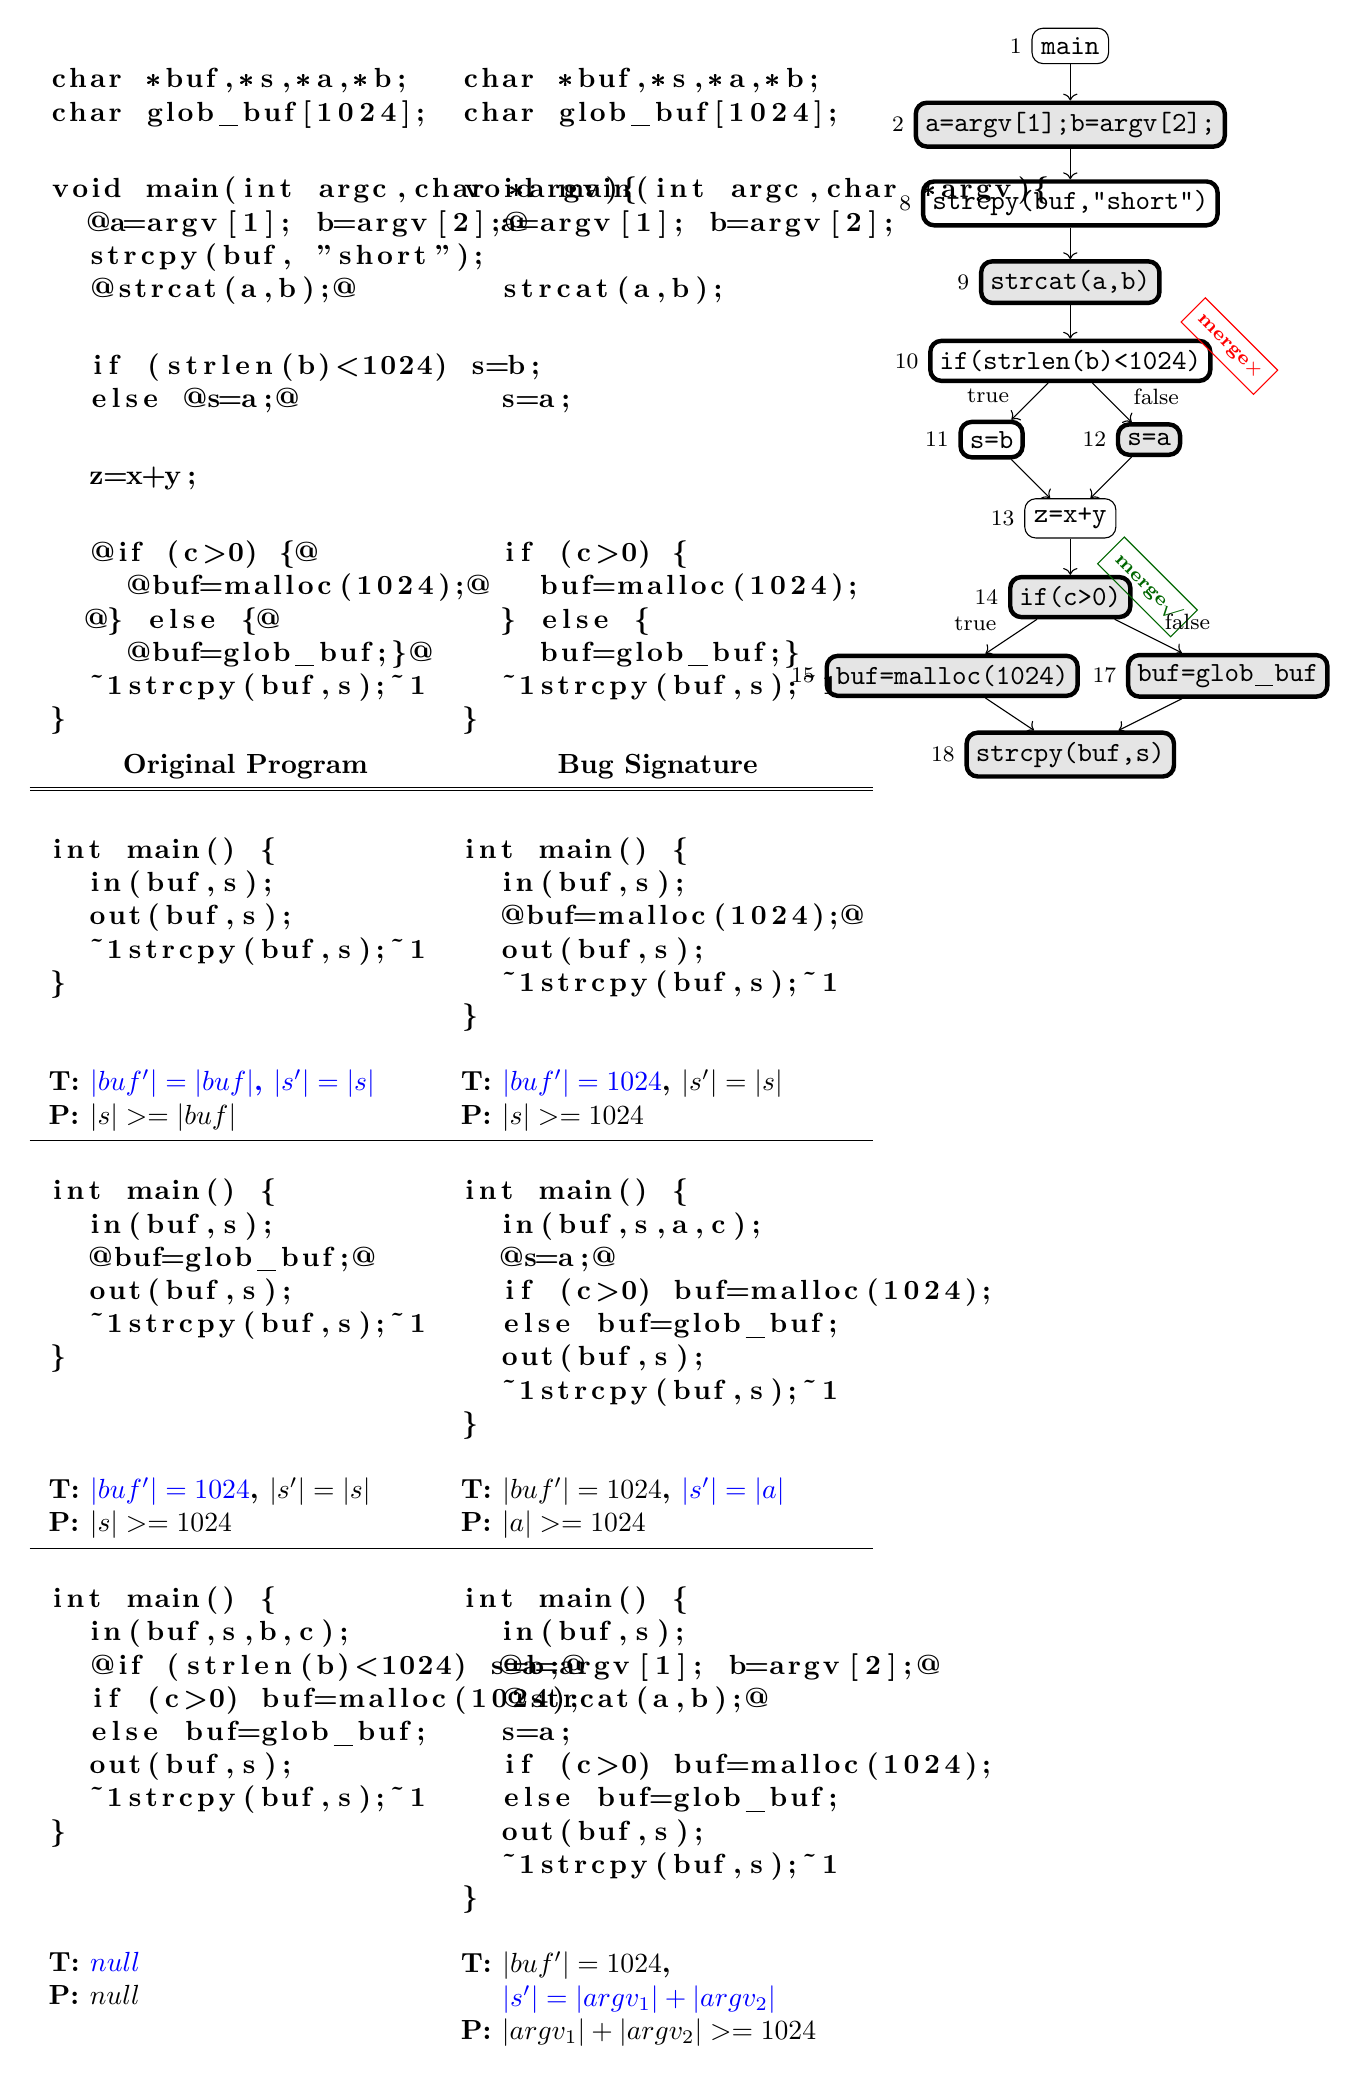
\begin{tikzpicture}[every label quotes/.style={left, font=\footnotesize},
      cfg/.style={draw,rectangle,rounded corners},
      tf/.style={text=\scriptsize},
      trans/.style={align=center,draw,rounded corners,rectangle
        split,rectangle split parts=2,draw,dashed,fill=gray!10!white,minimum width=5cm,font=\scriptsize\bfseries},
      bench/.style={draw,fill=gray!20!white},
      slice/.style={draw,ultra thick},
      merge label/.style={red,font=\scriptsize\bfseries,draw,rotate=-45,label position=40},
      every label/.style={font=\normalsize},
      num/.style={draw,circle},
      label position={0},
      font=\bfseries,
      ]

    \graph[grow down, branch right,
      nodes={draw,rectangle,rounded corners},
      ->
      % draw,
      ] {main/\texttt{main}["1"]
      -> "\texttt{a=argv[1];b=argv[2];}"[bench, slice, "2"]
      -> strcpy/"\texttt{strcpy(buf,"short")}"[slice,"8"]
      -> "\texttt{strcat(a,b)}"[bench,slice,"9"]
      -> "\texttt{if(strlen(b)<1024)}"[slice,"10",
        label={[merge label,shift={(6mm,9mm)}]merge$\times$}]
      -> [edge quotes={auto,pos=0.8,font=\footnotesize}]
      {
        "\texttt{s=b}"[slice,shift={(-1,0)}, > "true"',"11"],
        "\texttt{s=a}"[bench,slice,> "false","12"]
      }
      -> "\texttt{z=x+y}"["13"]
      -> c8/"\texttt{if(c>0)}"[bench,slice,"14",
        label={[merge label,shift={(-1mm,1mm)},green!40!black]merge$\surd$}]
      -> [edge quotes={auto, pos=0.6,font=\footnotesize}]
      {
        "\texttt{buf=malloc(1024)}"[bench,slice,shift={(-1.5,0)},> "true"',"15"],
        "\texttt{buf=glob_buf}"[shift={(1,0)},bench,slice,> "false","17"]}
      -> poi/"\texttt{strcpy(buf,s)}"[bench,slice,"18"]
    };
    
    \matrix (full) [
      left=2.5cm of main.north,
      matrix anchor=north east,
      every node/.style={
        % draw,
        inner ysep=0,
        text width=5cm,
        % inner xsep=10pt,
      },
      % column sep=3pt,
      anchor=north west,
      every label quotes/.style={below,font=\footnotesize},
      % align=center,
      % column sep=10pt,
      % draw
      ] {

      %% I'm going to split the code into parts

      \node {
\begin{lstlisting}
char *buf,*s,*a,*b;
char glob_buf[1024];
\end{lstlisting}        
      };&
      \node {
        \begin{lstlisting}
char *buf,*s,*a,*b;
char glob_buf[1024];
\end{lstlisting}
      };\\
      \node {
        \begin{lstlisting}
void main(int argc,char *argv){
  @a=argv[1]; b=argv[2];@
  strcpy(buf, "short");
  @strcat(a,b);@
\end{lstlisting}
      };&
      \node {
        \begin{lstlisting}
void main(int argc,char *argv){
  a=argv[1]; b=argv[2];

  strcat(a,b);
\end{lstlisting}
      };\\
      \node {
        \begin{lstlisting}
  if (strlen(b)<1024) s=b;
  else @s=a;@
\end{lstlisting}
      };&
      \node {
\begin{lstlisting}

  s=a;
\end{lstlisting}
      };\\
      \node {
        \begin{lstlisting}
  z=x+y;
\end{lstlisting}
      };&
      \node {
        \begin{lstlisting}
\end{lstlisting}
      };\\
      \node {
        \begin{lstlisting}
  @if (c>0) {@
    @buf=malloc(1024);@
  @} else {@
    @buf=glob_buf;}@
  ~1strcpy(buf,s);~1
}
\end{lstlisting}
      };&
      \node {
        \begin{lstlisting}
  if (c>0) {
    buf=malloc(1024);
  } else {
    buf=glob_buf;}
  ~1strcpy(buf,s);~1
}
\end{lstlisting}
      };\\
      \node [align=center] {
        Original Program
      };&
      \node [align=center] {
        Bug Signature
      };\\
    };
    % \draw (0,0) grid (10,10);
    \draw [double] (full.south west) -- (full.south east);

    \matrix (gen) [
      matrix anchor=north west,
      below=0pt of full.south west,
      % draw,
      % matrix of nodes,
      every node/.style={
        text width=5cm,
        % inner sep=0,
        align=left,
        % draw
      }
      ] {
      \node {
\begin{lstlisting}
int main() {
  in(buf,s);
  out(buf,s);
  ~1strcpy(buf,s);~1
}
\end{lstlisting}        
      };&
      \node {
\begin{lstlisting}
int main() {
  in(buf,s);
  @buf=malloc(1024);@
  out(buf,s);
  ~1strcpy(buf,s);~1
}
\end{lstlisting}        
      };\\
      \node  (t1) {
        T: {\color{blue}$|buf'|=|buf|$, $|s'|=|s|$}\\
        P: $|s| >= |buf|$
      };&
      \node {
        T: {\color{blue}$|buf'|=1024$}, $|s'|=|s|$\\
        P: $|s| >= 1024$
      };\\
      \node {
\begin{lstlisting}
int main() {
  in(buf,s);
  @buf=glob_buf;@
  out(buf,s);
  ~1strcpy(buf,s);~1
}
\end{lstlisting}        
      };&
      \node {
\begin{lstlisting}
int main() {
  in(buf,s,a,c);
  @s=a;@
  if (c>0) buf=malloc(1024);
  else buf=glob_buf;
  out(buf,s);
  ~1strcpy(buf,s);~1
}
\end{lstlisting}        
      };\\
      \node (t2) {
        T: {\color{blue}$|buf'|=1024$}, $|s'|=|s|$\\
        P: $|s| >= 1024$
      };&
      \node {
        T: $|buf'|=1024$, {\color{blue}$|s'|=|a|$}\\
        P: $|a| >= 1024$
      };\\
      \node {
        \begin{lstlisting}
int main() {
  in(buf,s,b,c);
  @if (strlen(b)<1024) s=b;@
  if (c>0) buf=malloc(1024);
  else buf=glob_buf;
  out(buf,s);
  ~1strcpy(buf,s);~1
}
\end{lstlisting}
      };&
      \node {
\begin{lstlisting}
int main() {
  in(buf,s);
  @a=argv[1]; b=argv[2];@
  @strcat(a,b);@
  s=a;
  if (c>0) buf=malloc(1024);
  else buf=glob_buf;
  out(buf,s);
  ~1strcpy(buf,s);~1
}
\end{lstlisting}
      };\\
      \node {
        T: {\color{blue}$null$}\\
        P: $null$
      };&
      \node {
        T: $|buf'|=1024$,\\
        {\color{white}T:} {\color{blue}$|s'|=|argv_1|+|argv_2|$}\\
        P: $|argv_1|+|argv_2|>=1024$
      };\\
    };

    % \draw (gen-1-1) -- (gen-1-2);
    \draw (t1.south -| gen.west) -- (t1.south -| gen.east);
    \draw (t2.south -| gen.west) -- (t2.south -| gen.east);
    
  \end{tikzpicture}
\end{figure*}









\begin{figure*}[ht!]
  \centering
  \begin{tikzpicture}[
      cfg/.style={draw,rectangle,rounded corners},
      tf/.style={text=\scriptsize},
      trans/.style={align=center,draw,rounded corners,rectangle
        split,rectangle split parts=2,draw,dashed,fill=gray!10!white,minimum width=5cm,font=\scriptsize\bfseries},
      bench/.style={draw,fill=gray!20!white},
      slice/.style={draw,ultra thick},
      merge label/.style={red,font=\scriptsize\bfseries,draw,rotate=-45,label position=40},
      every label/.style={font=\normalsize},
      num/.style={draw,circle},
      label position={0},
      font=\bfseries,
      ->
      ]

    \begin{scope}[every label quotes/.style={left}]
      \graph[grow down, branch right,
        nodes={draw,rectangle,rounded corners}
        ] {"\texttt{main}"["1"]
        -> "\texttt{a=argv[1];b=argv[2];}"["2"]
        -> "\texttt{func()}"["3"]
        -> thefor/"\texttt{for(p=a;*p!='\textbackslash0';p++)}"[slice,"4"]
        -> [edge quotes={auto,font=\footnotesize}] "\texttt{*p='y'}"[slice,"5",> "true"']
        -> forif/"\texttt{if(p)}"[slice,"6"]
        -> [edge quotes={auto,font=\footnotesize}] "\texttt{break}"[slice,"7",> "true"]
        -> strcpy/"\texttt{strcpy(buf,"short")}"[slice,"8"]
        -> "\texttt{strcat(a,b)}"[bench,slice,"9"]
        -> "\texttt{if(strlen(b)<1024)}"[slice,"10",label={[merge label,shift={(6mm,9mm)}]merge$\times$}]
        -> [edge quotes={auto,pos=0.8,font=\footnotesize}] {"\texttt{s=b}"[slice,shift={(-1,0)}, > "true"',"11"],
          "\texttt{s=a}"[bench,slice,> "false","12"]
        }
        -> "\texttt{z=x+y}"["13"]
        -> c8/"\texttt{if(c>8)}"[slice,"14",label={[merge label,shift={(-1mm,1mm)},green!40!black]merge$\surd$}]
        -> [edge quotes={auto, pos=0.6,font=\footnotesize}]
        {"\texttt{p=malloc(1024)}"[bench,slice,shift={(-1.5,0)},> "true"',"15"]
          -> "\texttt{buf=p}"[bench,slice,shift={(-1.5,0)},"16"],
          "\texttt{buf=buf2}"[shift={(1,0)},bench,slice,> "false","17"]}
        -> poi/"\texttt{strcpy(buf,s)}"[bench,slice,"18"]
      };
      \draw (forif) to[bend left,"false" auto, pos=0.5,font=\footnotesize] ($(thefor.south)+(-1.5,0)$);
      \draw ($(thefor.south)+(1,0)$) to[bend left, "false" auto, pos=0.3,font=\footnotesize] ($(strcpy.north)+(1,0)$);
    \end{scope}


    % \draw (poi) -- (c8);

    % \matrix[draw=red] {
    % \node {a}; & \node {b}; & \node {c};\\
    % };

    %   \matrix [draw=red,column sep=1cm]
    %   {
    %   \node {8}; & \node{1}; & \node {6}; \\
    %   \node {3}; & \node{5}; & \node {7}; \\
    %   \node {4}; & \node{9}; & \node {2}; \\
    % };

    \matrix[
      every node/.style={anchor=north},
      anchor=south,
      % above=of poi.south,
      % shift={(0,-1.5)},
      every label quotes/.style={below,font=\footnotesize},
      % every label/.style={font=\footnotesize},
      align=center
      ] {
      \node (input)
      [shift={(0.4,0)},label={[font=\scriptsize,
            % draw,decorate, decoration={random steps,segment length=3pt,amplitude=1pt},fill=gray!20!white
            ]above:Input: Buggy Program}] {
\begin{lstlisting}[
label={lst-overview-example},
basicstyle=\scriptsize\ttfamily,
numbers=left
]
char *buf,*s,*a,*b;
void main(int argc,char *argv){
  @a=argv[1]; b=argv[2];@
  func();
  for(char *p=a;*p!='\0';p++){
    *p='y'; if (p) break;}
  strcpy(buf, "short");
  @strcat(a,b);@
  if (strlen(b)<1024) s=b;
  else @s=a;@
  z=x+y;
  @if (c>8)@ {
    @p=malloc(1024); buf=p;@
  } @else@ {
    @buf=buf2;@}
  ~1strcpy(buf,s);~1
}
\end{lstlisting}
      }; &[7cm]
      \node (output)
      [shift={(0.4,0)},label={[font=\scriptsize,
            % draw,decorate, decoration={random steps,segment length=3pt,amplitude=1pt},fill=gray!20!white
            ]above:Output: Bug Signature}] {
\begin{lstlisting}[
label={lst-overview-example},
basicstyle=\scriptsize\ttfamily,
numbers=left
]
char *buf,*s,*a,*b;
void main(int argc,char *argv){
  char *a=argv[1];
  char *b=argv[2];
  strcat(a,b);
  s=a;
  if (c>8) {
    p=malloc(1024); buf=p;
  } else {
    buf=buf2;}
  ~1strcpy(buf,s);~1
}
\end{lstlisting}
      };\\
      \node {}; & \node {};\\
      \node {}; & \node {};\\
      \node (maincallbartrans)[trans,"2"] {
        \texttt{\color{red}\underline{len($argv_1$)+len($argv_2$)>1024;}}
        \nodepart{two}
        \texttt{sizeof(buf')=1024;}\\
        \texttt{\color{blue}\underline{len(s')=len($argv_1$)+len($argv_2$)};}
      }; &
      \node (strcattrans)[trans,"3-9"] {
        \texttt{len(a)+len(b)>1024;}
        \nodepart{two}
        \texttt{sizeof(buf')=1024;}\\
        \texttt{\color{blue}\underline{len(s')=len(a)+len(b)};}
      }; \\
      % \node (strcattrans)[trans,"11-15"] {
      % \texttt{{\color{blue}\underline{len(a)+len(b)}}>1024;}
      % \nodepart{two}
      % \texttt{sizeof(buf')=1024;}\\
      % \texttt{len(s')={\color{blue}\underline{len(a)+len(b)}};}
      % }; &

      \node (iflentrans1)[trans,"10-(1)"] {
        $\emptyset$
        \nodepart{two}
        $\emptyset$
      }; &

      \node (iflentrans2)[trans,"10-(2)",label={[merge label,label distance=-5mm,shift={(10mm,10mm)},overlay]"merge$\times$"}] {
        \texttt{len(a)>1024;}
        \nodepart{two}
        \texttt{size(buf')=1024;}\\
        \texttt{len(s')=len(a);}
      }; \\

      \node (sbtrans)[trans,"11"] {
        \texttt{len(b)>1024;}
        \nodepart{two}
        \texttt{size(buf')=1024;}\\
        \texttt{\color{blue}\underline{len(s')=len(b);}}
      }; &
      \node (satrans)[trans,"12"] {
        \texttt{len(a)>1024;}
        \nodepart{two}
        \texttt{size(buf')=1024;}\\
        \texttt{\color{blue}\underline{len(s')=len(a)};}
      }; \\

      \node (c8trans) [trans,"14",label={[merge label,green!40!black,shift={(7mm,8mm)},overlay]"merge$\surd$"}] {
        \texttt{len(s)>1024;}
        \nodepart{two}
        \texttt{\color{blue}\underline{size({buf'})=1024;}}\\
        \texttt{len(s')=len(s);}
      }; &

      \node (buf2trans) [trans,"17"] {
        \texttt{len(s)>size(buf2);}
        \nodepart{two}
        \texttt{\color{blue}{\underline{size({buf'})=size(buf2);}}}\\
        \texttt{len(s')=len(s);}
      }; \\

      \node (malloctrans) [trans,"15"] {
        \texttt{len(s)>1024;}
        \nodepart{two}
        \texttt{\color{blue}{\underline{size({buf'})=1024;}}}\\
        \texttt{len(s')=len(s);}
      }; &
      \node (poitrans)[trans,"18"] {
        \texttt{len(s)>size(buf);}
        \nodepart{two}
        \texttt{\color{blue}{\underline{size({buf'})=size(buf);}}}\\
        \texttt{len(s')=len(s);}
      }; \\

      \node (assignbuftrans) [trans,"16"] {
        \texttt{len(s)>size(p);}
        \nodepart{two}
        \texttt{\color{blue}\underline{size({buf'})=size(p);}}\\
        \texttt{len(s')=len(s);}
      }; &

      \node (feature)[align=left,font=\scriptsize\bfseries,draw,decorate, decoration={random steps,segment length=3pt,amplitude=1pt},fill=gray!20!white,shift={(0,-0.3)}] {
        Query for Demand: \\\texttt{len(s')>size(buf')}
      };\\
    };
  \end{tikzpicture}
\end{figure*}

\end{document}
